\documentclass[25pt, a0paper, portrait]{tikzposter}
\usepackage[utf8]{inputenc}
\usepackage[T1]{fontenc}
\usepackage{lmodern}
\usepackage{amsmath}
\usepackage{amsfonts}
\usepackage{amssymb}
\usepackage{graphicx}
\usepackage{tikz}
\usetikzlibrary{shapes,arrows,positioning,fit,backgrounds,calc}

\definecolor{bleu303}{RGB}{0,62,92}
\definecolor{rouge485}{RGB}{213,43,30}
\definecolor{bleu315}{RGB}{0,104,128}


\title{
    \parbox{\linewidth}{
        \begin{minipage}{0.2\linewidth}
            \centering
            \colorbox{white}{
\includegraphics[height=3.5cm]{polytechnique-logohori.pdf}}
        \end{minipage}%
        \begin{minipage}{0.6\linewidth}
            \centering
            \textbf{AudioConditioner}\\[0.2em] \Large Models \& Training
        \end{minipage}%
        \begin{minipage}{0.2\linewidth}
            \centering
            \colorbox{white}{
\includegraphics[height=3.8cm]{polytechnique-armes.pdf}}
        \end{minipage}
    }
}
\author{}
\institute{CSC\_52002\_EP - Multimodal generative AI}

\usetheme{Default}
\useblockstyle{Minimal}
\colorlet{backgroundcolor}{white}
\colorlet{titlebgcolor}{bleu303}
\colorlet{titlefgcolor}{white}
\colorlet{blocktitlebgcolor}{white}
\colorlet{blocktitlefgcolor}{rouge485}
\colorlet{blockbodybgcolor}{white}
\colorlet{blockbodyfgcolor}{black}

\begin{document}

\maketitle

\node[fill=bleu303, text=white, minimum width=\paperwidth, minimum height=2.5cm, anchor=south] at (current page.south) {
    \begin{minipage}{0.9\textwidth}
        \bfseries\small 
        Keyvan Attarian \& Baptiste Arnaudo \hfill Ecole polytechnique, X23
    \end{minipage}
};

\begin{columns}

\column{0.5}

\block{\MakeUppercase{Introduction \& The Descriptor Model}}{
    \vspace{-1cm}
    
\includegraphics[width=0.6\linewidth]{polytechnique-filetlongrouge.pdf}\\[0.5cm]
    The \textbf{Audio\-Conditioner} is a high-level multimodal model that bridges the gap between visual/textual semantics and music generation utilizing \textbf{BLIP} for image captioning and the \textbf{CLAP} text encoder for semantic embeddings.
    \vspace{0.5cm}
    
    The core innovation is our \textbf{Descriptor Model}, which is the \textit{only trainable component in the entire architecture}. All other models (BLIP, CLAP, Stable Audio) are kept completely frozen. The Descriptor acts as a multi-task learning bridge, mapping the CLAP text embedding through a shared neural backbone into 12 discrete and continuous musical attributes.
    \vspace{0.5cm}
    
    The generated attributes are structurally combined within a \texttt{Music\-Descriptor} object. This object then programmatically generates the final descriptive text prompt fed into \textbf{Stable Audio} (which has a 47-second generation limit). Finally, to ensure strict semantic alignment, we generate $N$ candidates and re-rank them using \textbf{Cosine Similarity} against the CLAP text embedding.
}

\block{\MakeUppercase{The MusicDescriptor Schema}}{
    \vspace{-1cm}
    
\includegraphics[width=0.6\linewidth]{polytechnique-filetlongrouge.pdf}\\[0.5cm]
    {\color{bleu315}\LARGE\bfseries\sffamily Classification Attributes}
    \begin{itemize}
        \item[\color{bleu303}\textbullet] \textbf{Mood} \textit{($\rightarrow$ Multi-Label List)}: Emotional states (e.g., dark, epic, melancholic).
        \item[\color{bleu303}\textbullet] \textbf{Key/Mode} \textit{($\rightarrow$ Single-Label)}: The musical scale used (e.g., major, minor).
        \item[\color{bleu303}\textbullet] \textbf{Instrumentation} \textit{($\rightarrow$ Multi-Label List)}: Active instruments (e.g., strings, synth).
        \item[\color{bleu303}\textbullet] \textbf{Rhythm Style} \textit{($\rightarrow$ Single-Label)}: Overall rhythmic feel (e.g., sparse, pulsing).
        \item[\color{bleu303}\textbullet] \textbf{Structure} \textit{($\rightarrow$ Single-Label)}: Internal song progression (e.g., slow-build).
        \item[\color{bleu303}\textbullet] \textbf{Production Style} \textit{($\rightarrow$ Multi-Label List)}: Mixing/Genre aesthetic (e.g., cinematic).
        \item[\color{bleu303}\textbullet] \textbf{Dynamics Profile} \textit{($\rightarrow$ Single-Label)}: Volume progression (e.g., gradual build).
    \end{itemize}
    \vspace{0.5cm}
    {\color{bleu315}\Large\scshape Regression Attributes}
    \begin{itemize}
        \item[\color{bleu303}\textbullet] \textbf{Energy} \textit{($[0.0, 1.0]$)}: Overall intensity level (0.0 = very calm, 1.0 = very energetic).
        \item[\color{bleu303}\textbullet] \textbf{Valence} \textit{($[0.0, 1.0]$)}: Emotional polarity (0.0 = very negative/sad, 1.0 = very positive/happy).
        \item[\color{bleu303}\textbullet] \textbf{Tempo} \textit{($[50, 180]$ BPM)}: Beats per minute, strictly normalized to $[0.0, 1.0]$.
        \item[\color{bleu303}\textbullet] \textbf{Harmonic Tension} \textit{($[0.0, 1.0]$)}: Chord dissonance (0.0 = very consonant, 1.0 = very dissonant).
        \item[\color{bleu303}\textbullet] \textbf{Texture Density} \textit{($[0.0, 1.0]$)}: Number of simultaneous elements (0.0 = very minimal, 1.0 = very layered).
    \end{itemize}
}

\block{\MakeUppercase{Framework Architecture}}{
    \vspace{-1cm}
    
\includegraphics[width=0.6\linewidth]{polytechnique-filetlongrouge.pdf}\\[0.5cm]
    \begin{center}
    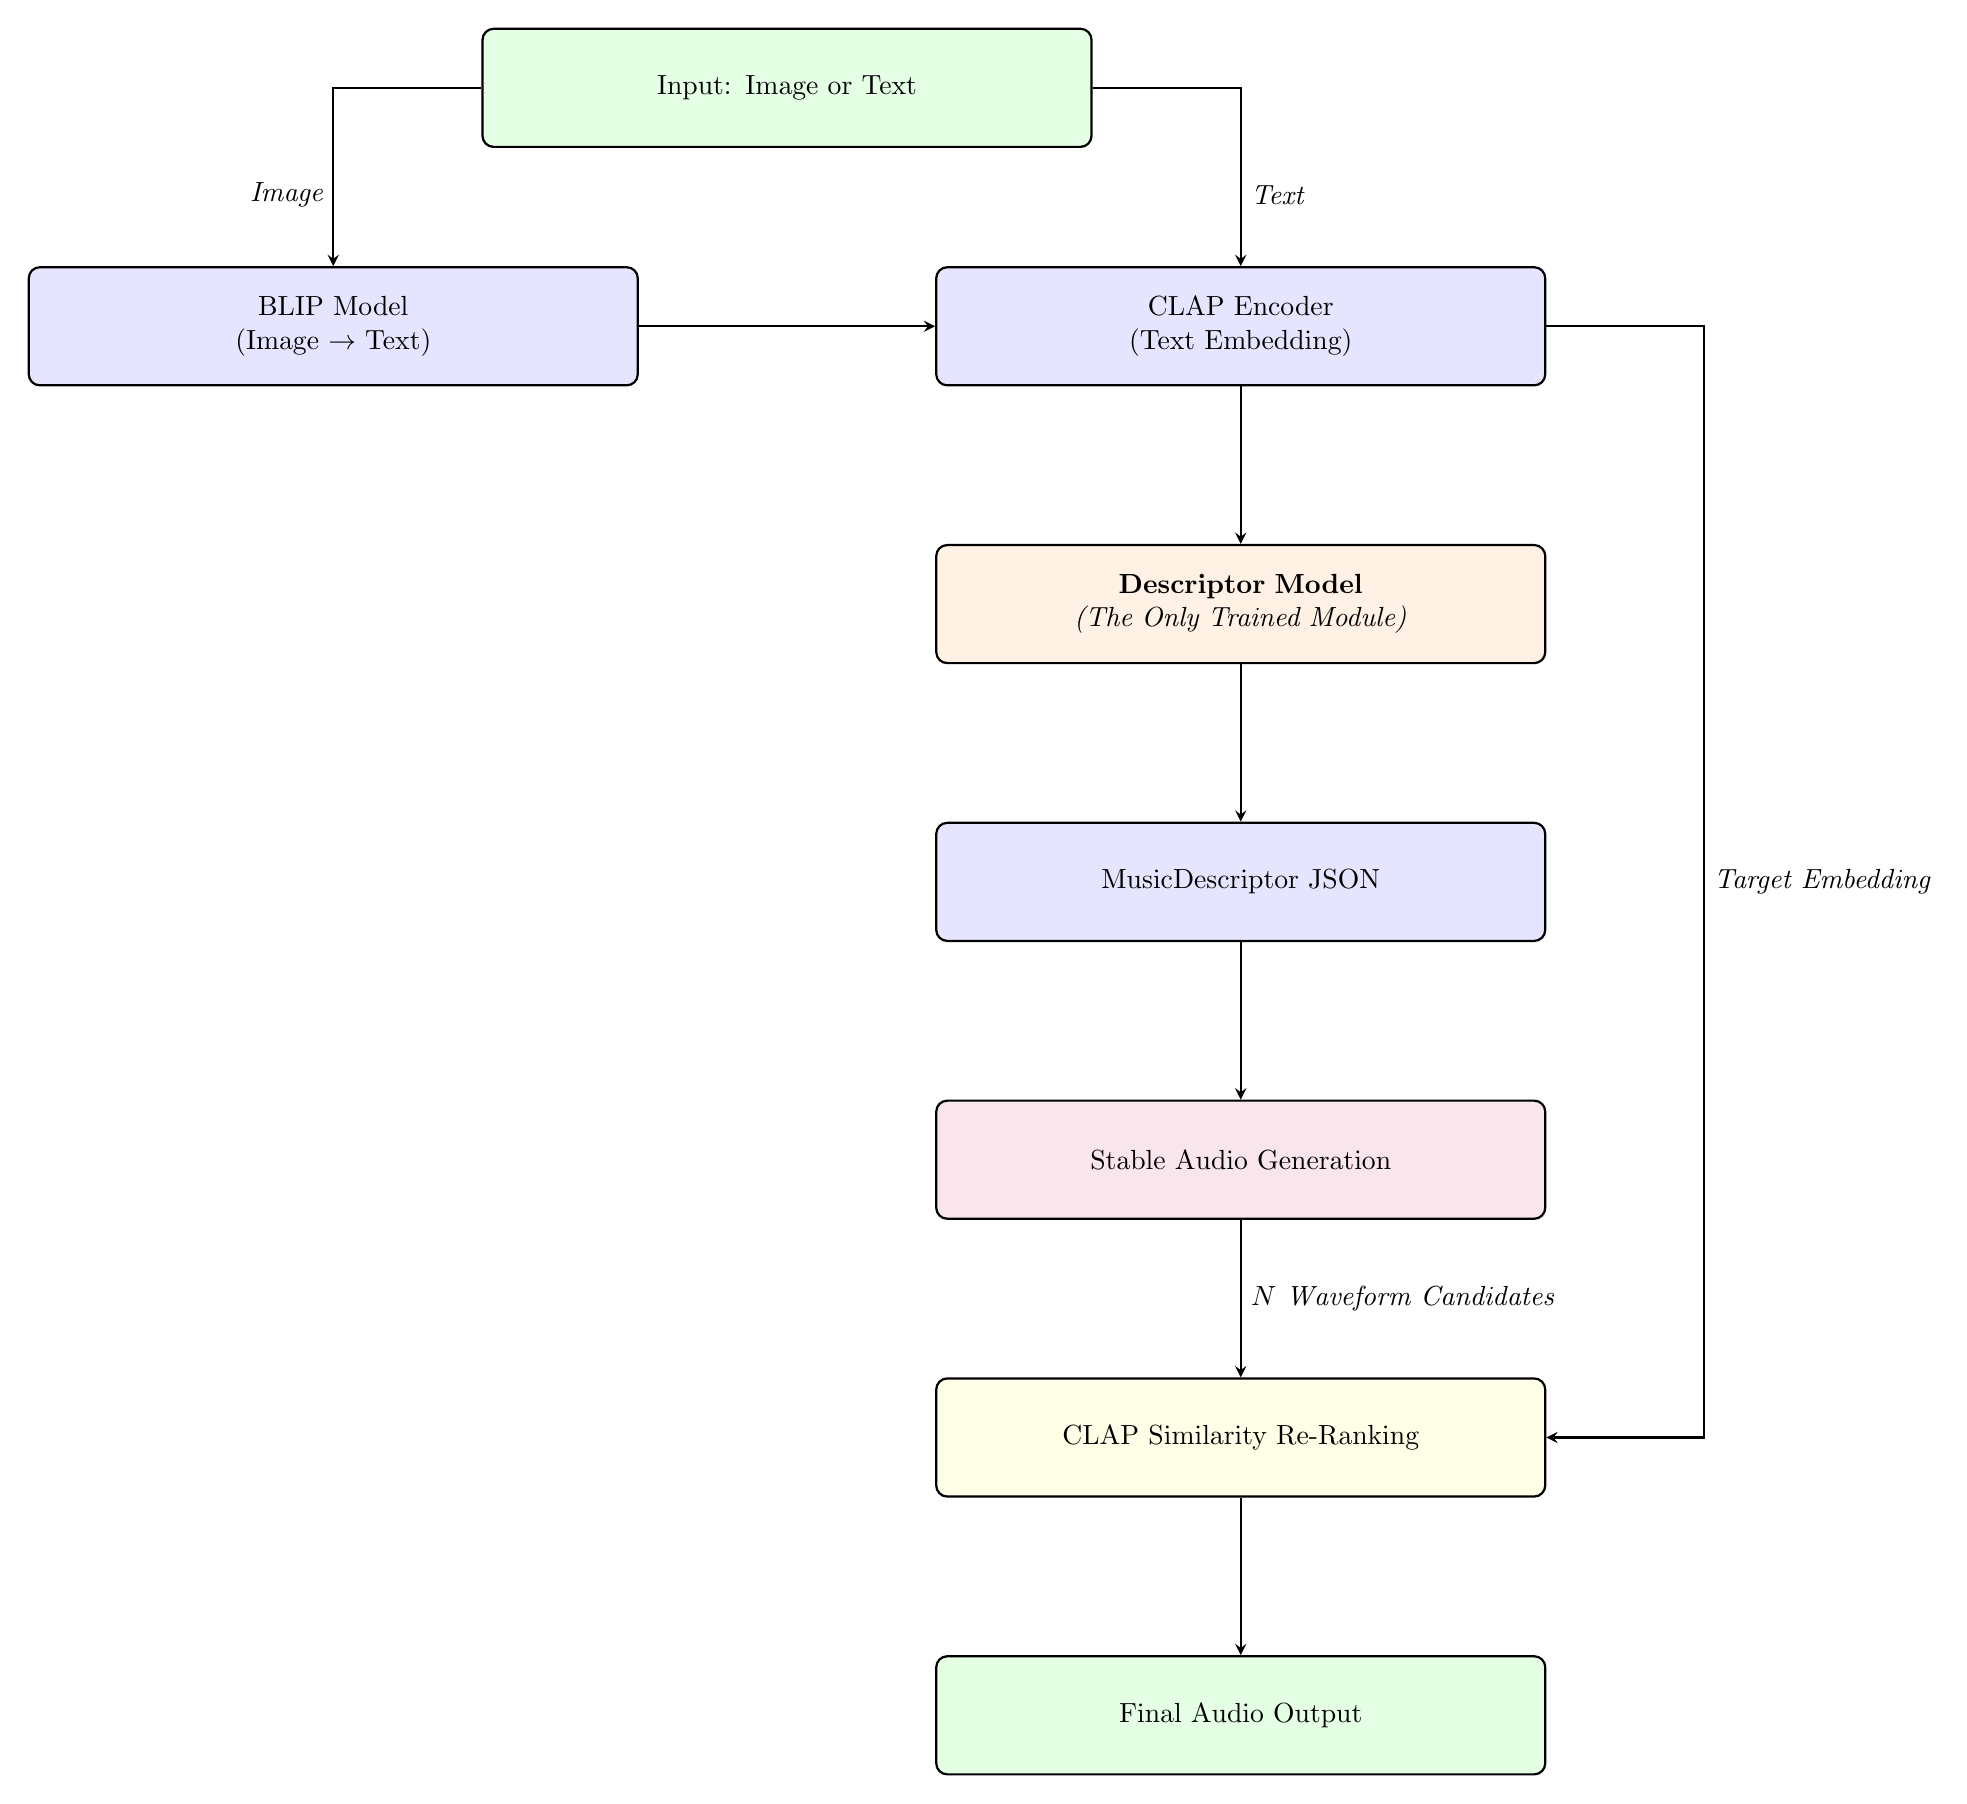
\begin{tikzpicture}[
        node distance=2cm and 2cm,
        box/.style={rectangle, draw=black, thick, fill=blue!10, text width=7.5cm, align=center, rounded corners, minimum height=1.5cm},
        arrow/.style={->, thick, >=stealth}
    ]
    
    \node[box, fill=green!10] (input) {Input: Image or Text};
    \node[box] (blip) [below left=1.5cm and -2cm of input] {BLIP Model \\ (Image $\rightarrow$ Text)};
    \node[box] (clap_text) [below right=1.5cm and -2cm of input] {CLAP Encoder \\ (Text Embedding)};
    \node[box, fill=orange!10] (descriptor) [below=2cm of clap_text] {\textbf{Descriptor Model} \\ \textit{(The Only Trained Module)}};
    \node[box] (prompt) [below=2cm of descriptor] {MusicDescriptor JSON};
    \node[box, fill=purple!10] (stable) [below=2cm of prompt] {Stable Audio Generation};
    \node[box, fill=yellow!10] (rerank) [below=2cm of stable] {CLAP Similarity Re-Ranking};
    \node[box, fill=green!10] (output) [below=2cm of rerank] {Final Audio Output};

    \draw[arrow] (input) -| node[left, pos=0.8] {\itshape Image} (blip);
    \draw[arrow] (input) -| node[right, pos=0.8] {\itshape Text} (clap_text);
    \draw[arrow] (blip) -- (clap_text);
    \draw[arrow] (clap_text) -- (descriptor);
    \draw[arrow] (descriptor) -- (prompt);
    \draw[arrow] (prompt) -- (stable);
    \draw[arrow] (stable) -- node[right] {\itshape $N$ Waveform Candidates} (rerank);
    \draw[arrow] (clap_text.east) -- ++(2,0) |- node[right, near start] {\itshape Target Embedding} (rerank.east);
    \draw[arrow] (rerank) -- (output);
    
    \end{tikzpicture}
    \end{center}
}

\column{0.5}

\block{\MakeUppercase{Phase 1: Generative LLM Distillation}}{
    \vspace{-1cm}
    
\includegraphics[width=0.6\linewidth]{polytechnique-filetlongrouge.pdf}\\[0.5cm]
    Training the \textbf{Descriptor Model} required a large parallel corpus mapping natural language to the strict \texttt{Music\-Descriptor} format. We built this automatically through \textbf{Prompt Mixing} and \textbf{Teacher LLM Distillation}:
    \begin{itemize}
        \item \textbf{Data Generation:} Instead of using an LLM to write scenes, we procedurally generated millions of short scene combinations by randomly mixing predefined \textit{characters}, \textit{characteristics}, \textit{settings}, and \textit{emotional events} (e.g., \textit{"A lonely astronaut under a burning sunset discovers an unexpected opportunity."}).
        \item \textbf{Distillation:} We then prompted an LLM to act as an expert composer, taking these random scenes and outputting the deterministic JSON \texttt{Music\-Descriptor} (Mood, Tempo, etc.) fitting each scene.
        \item \textbf{Optimization:} The model was trained using an \texttt{AdaptedMusicDescriptorLoss} function (Cross-Entropy for categorical attributes and MSE for continuous target regressions).
    \end{itemize}
    \vspace{1cm}
    \begin{center}
        
\includegraphics[width=0.48\linewidth]{avg_loss.png}
        \hfill
        
\includegraphics[width=0.48\linewidth]{val_loss.png}
    \end{center}
}

\block{\MakeUppercase{Phase 2: Contextual Novel Fine-Tuning}}{
    \vspace{-1cm}
    
\includegraphics[width=0.6\linewidth]{polytechnique-filetlongrouge.pdf}\\[0.5cm]
    To support narrative audiobook generation (\textbf{ReadMusic}), we fine-tuned the model to handle longer contextual evolution:
    \begin{enumerate}
        \item \textbf{Novel Chunking:} Public domain novels data were split into consecutive paragraphs (up to 80 words max).
        \item \textbf{Target Generation:} The Teacher LLM assigned progressive \texttt{MusicDescriptors} respecting the storyline's emotional flow.
        \item \textbf{Fine-Tuning Outcomes:} The Descriptor internalizes literary context, preventing abrupt changes and enabling smooth, continuous emotional transitions for long-form reading.
    \end{enumerate}
}

\block{\MakeUppercase{Training Pipeline Overview}}{
    \vspace{-1cm}
    
\includegraphics[width=0.6\linewidth]{polytechnique-filetlongrouge.pdf}\\[0.5cm]
    \begin{center}
    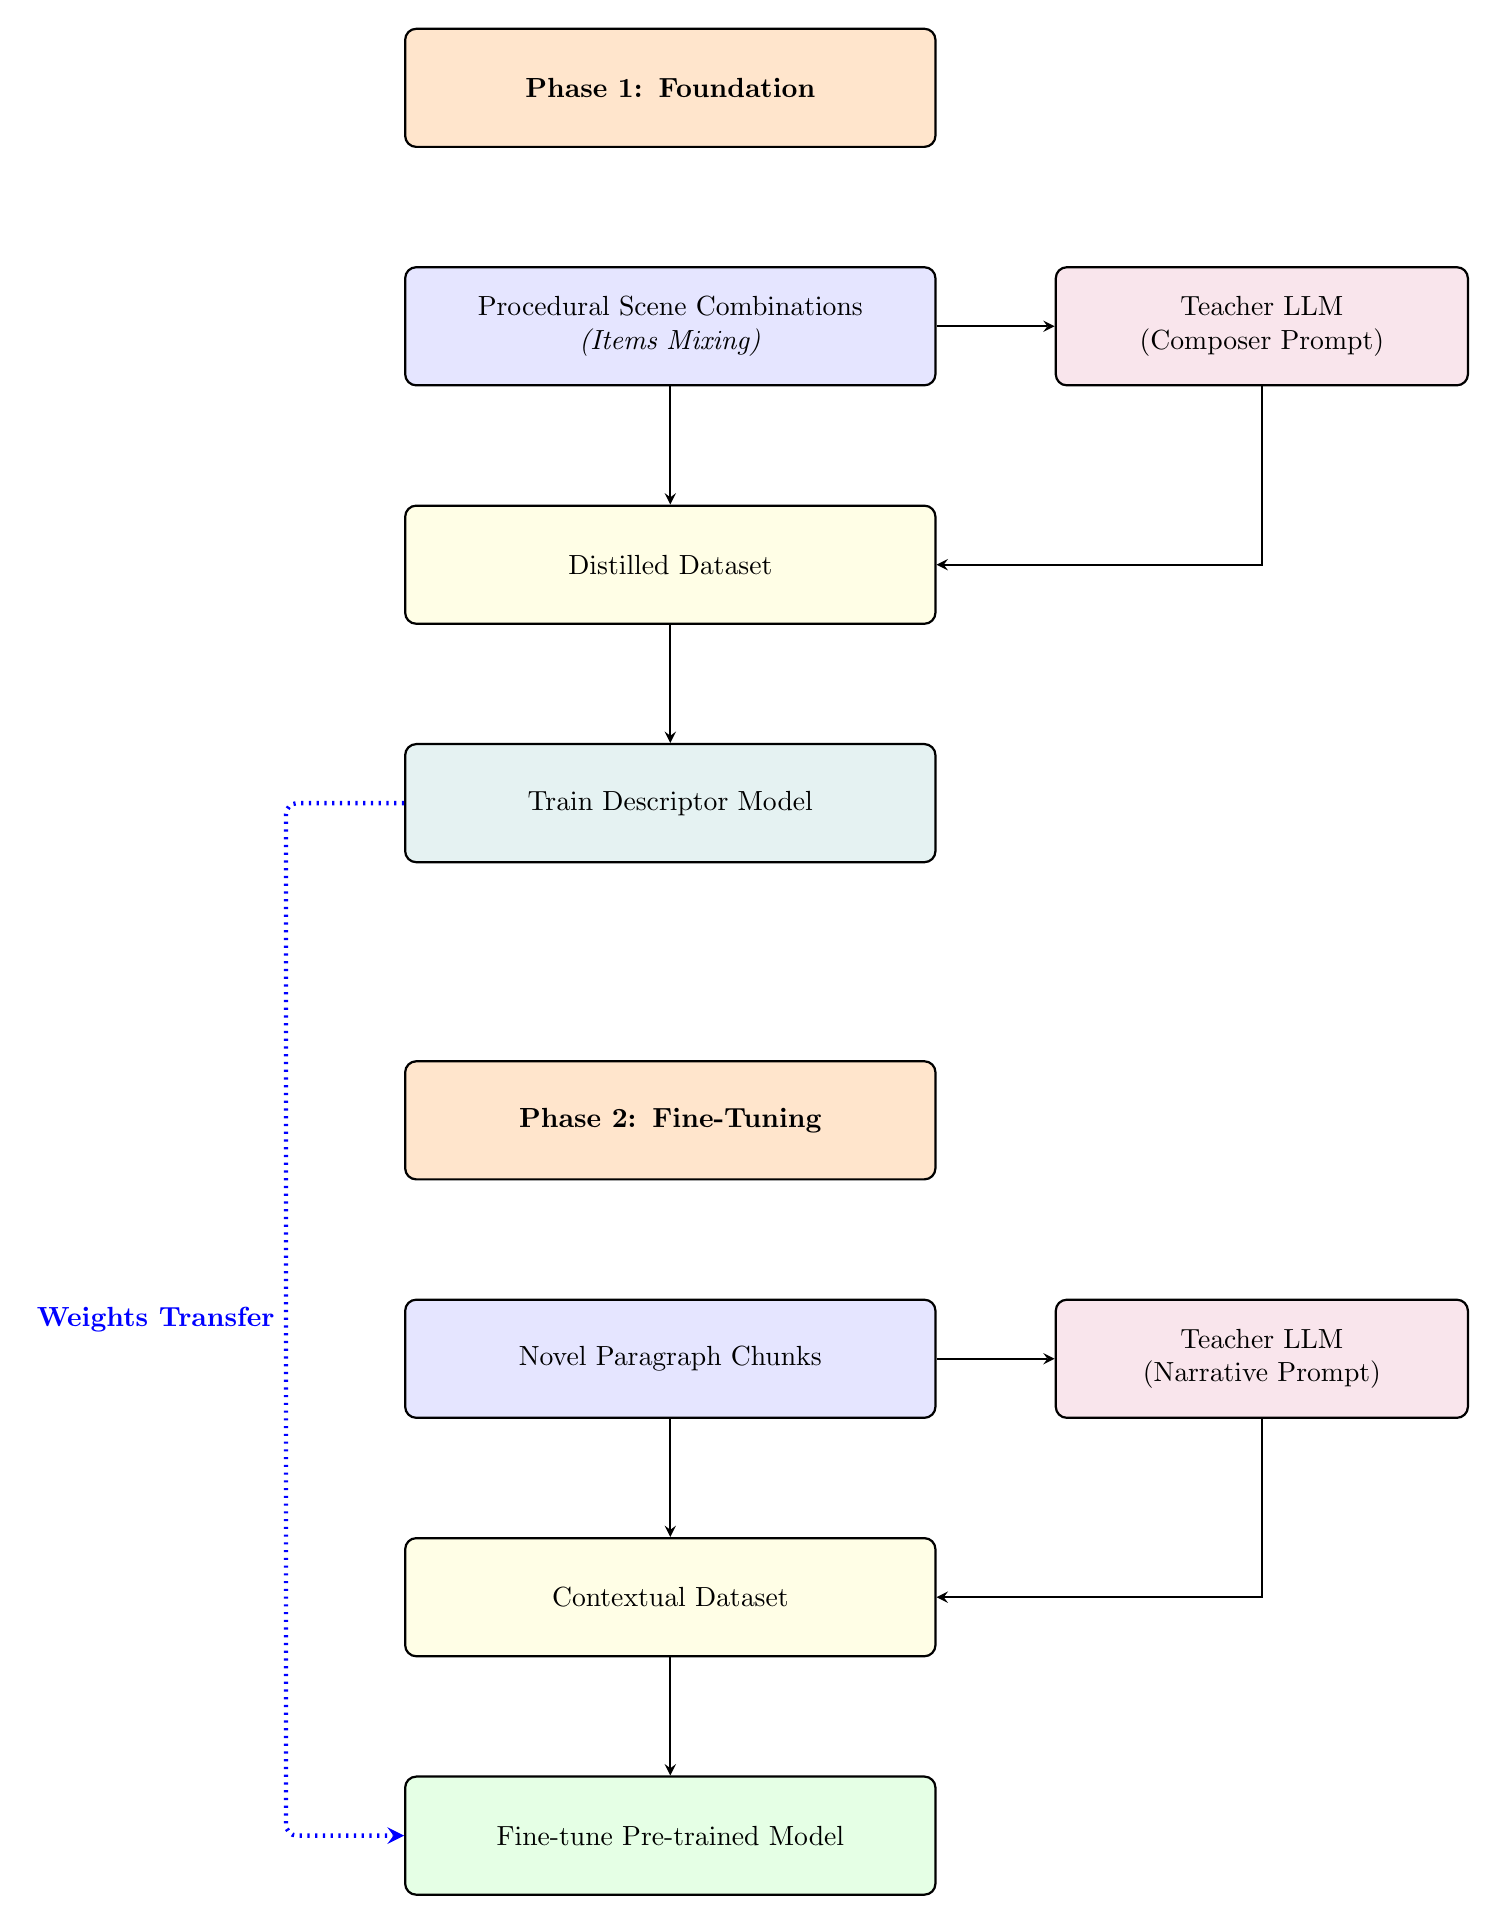
\begin{tikzpicture}[
        node distance=1.5cm and 1.5cm,
        box/.style={rectangle, draw=black, thick, fill=blue!10, text width=6.5cm, align=center, rounded corners, minimum height=1.5cm},
        llmbox/.style={rectangle, draw=black, thick, fill=purple!10, text width=5cm, align=center, rounded corners, minimum height=1.5cm},
        arrow/.style={->, thick, >=stealth}
    ]
    
    \node[box, fill=orange!20, font=\bfseries] (phase1) {Phase 1: Foundation};
    \node[box] (random_text) [below=of phase1] {Procedural Scene Combinations \\ \textit{(Items Mixing)}};
    \node[llmbox] (llm1) [right=of random_text] {Teacher LLM \\ (Composer Prompt)};
    \node[box, fill=yellow!10] (dataset1) [below=of random_text] {Distilled Dataset};
    \node[box, fill=teal!10] (train1) [below=of dataset1] {Train Descriptor Model};
    
    \draw[arrow] (random_text) -- (llm1);
    \draw[arrow] (llm1) |- (dataset1);
    \draw[arrow] (random_text) -- (dataset1);
    \draw[arrow] (dataset1) -- (train1);
    
    \node[box, fill=orange!20, font=\bfseries] (phase2) [below=of train1, yshift=-1cm] {Phase 2: Fine-Tuning};
    \node[box] (novel_text) [below=of phase2] {Novel Paragraph Chunks};
    \node[llmbox] (llm2) [right=of novel_text] {Teacher LLM \\ (Narrative Prompt)};
    \node[box, fill=yellow!10] (dataset2) [below=of novel_text] {Contextual Dataset};
    \node[box, fill=green!10] (train2) [below=of dataset2] {Fine-tune Pre-trained Model};
    
    \draw[arrow] (novel_text) -- (llm2);
    \draw[arrow] (llm2) |- (dataset2);
    \draw[arrow] (novel_text) -- (dataset2);
    \draw[arrow] (dataset2) -- (train2);
    \draw[arrow, dotted, ultra thick, blue, rounded corners] (train1.west) -- ++(-1.5,0) |- node[pos=0.25, left, font=\bfseries] {Weights Transfer} (train2.west);

    \end{tikzpicture}
    \end{center}
}

\end{columns}
\end{document}
